%-----------------------------------------------------------------------------%
\chapter{\babTiga}
%-----------------------------------------------------------------------------%
Apa itu Bab 3?


%-----------------------------------------------------------------------------%
\section{Contoh}
%-----------------------------------------------------------------------------%
\subsection{Subbab Contoh Satu}
%--------------
\lipsum[7]

\begin{enumerate}
	\item Tahap 1. \\ %\lstinputlisting[language=Java, caption=Contoh kode, label=code:sample]{assets/3-sample.java}
	Jelaskan teori menurut rujukan contoh \autocite{sahroni2018fikih} dengan semua nama penulis.

	\lipsum[6-8]

	\item Tahap 2.
\end{enumerate}

Tulis kesimpulan di sini. Contoh rujukan sitasi \autocite{UINJAKARTARoikhan2017} yang akan
ditampilkan pada halaman daftar pustaka.
Kembali merujuk \textcite{sahroni2018fikih} tetapi dengan kutipan langsung.

%------------
\subsection{Subbab Contoh Dua}
%-----------

\lipsum[55-57]

%---------------------------
\section{Metode Analisis Data}
%---------------------------

Data yang diperoleh akan dianalisis dengan menggunakan teknik analisis data kualitatif.
Menurut Bogdan \autocite{Sugiyono2008} analisis data adalah proses mencari dan menyusun
secara sistematis data yang diperoleh dari hasil wawancara, catatan lapangan, dan
bahan-bahan lain, sehingga  mudah dipahami, dan temuannya dapat diinformasikan kepada orang lain.
\ldots

\begin{figure}
\caption{Analisis Data Miles dan Huberman}
\centering
% 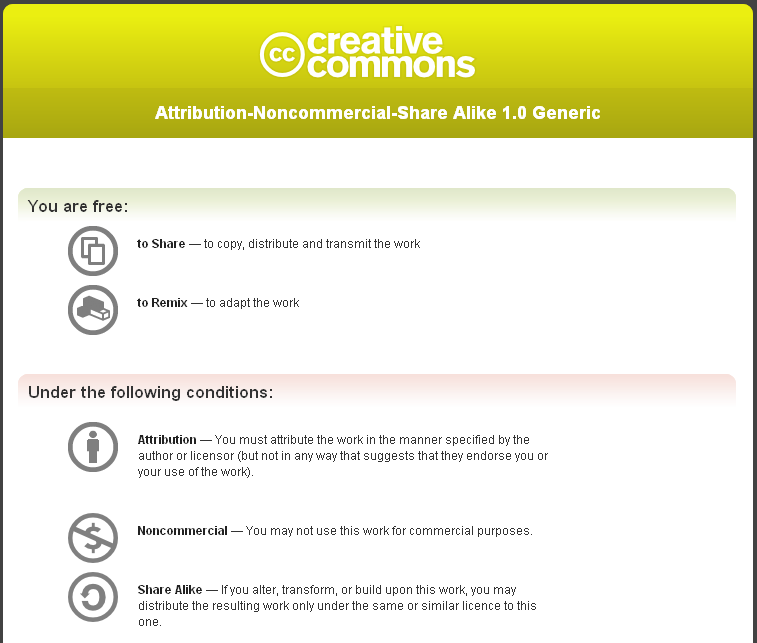
\includegraphics[width=0.6\textwidth]{assets/pics/creative_commons.png}
\begin{tikzpicture}
    \tikzset{node distance = 2.5cm}
    \tikzstyle{every node}=[thick, draw, ellipse, minimum width=100pt,inner sep=10pt,align=center]
    % Nodes
    \node[text width=3.5cm] (node1) {Data Collection};
    \node[text width=3cm] (node2) [right = 2cm of node1] {Data Display};
    \node[text width=2cm, inner sep=5pt,below = 0.3cm and 0.1cm of node1, xshift=3cm] (node3) {Data Reduction};
    \node[rectangle, rounded corners=2mm,text width=6.5cm, below=3.5 cm of node1, xshift=2.4cm] (node4) {Conclusions: drawing/verifying};

    % Arrows
    \draw[-{Latex[length=2mm]}] (node1) -- (node2);
    \draw[-{Latex[length=2mm]}] (node1) -- (node3);
    \draw[{Latex[length=2mm]}-] (node1) -- (node4);
    \draw[{Latex[length=2mm]}-{Latex[length=2mm]}] (node2) -- (node4);
    \draw[{Latex[length=2mm]}-{Latex[length=2mm]}] (node2) -- (node3);
    \draw[{Latex[length=2mm]}-{Latex[length=2mm]}] (node3) -- (node4);

\end{tikzpicture}
{\footnotesize Sumber: \textcite{Sugiyono2008}\par}
\end{figure}
